\section{Comparacion Round-Robin/FCFS}

\subsection{FCFS}

El FCFS "First Come, First Served", como su nombre sugiere es un scheduler con una política de estilo FIFO, es decir que la primera tarea en la cola de tareas será la primera en pasar al estado \textit{runing} y la primera en finalizar (en el núcleo en el que fue asignada). Mas específicamente, dado como parametro el \textit{switch\_cost} y un número $n$ de cores, asigna las primeras $n$ tareas en estar en estado \textit{ready} a los $n$ núcleos disponibles (asignando la tarea \textit{IDLE} para aquellos para los cuales no haya alguna tarea lista), y permitiendoles permanecer en \textit{runing} sin conmutarlas con otras hasta que estas primeras finalicen; de modo que lidiada con cada tarea una sóla vez, y sin ningun tipo de desalojo intermedio. 

\subsection{Round-Robin}

El Round-Robin es un scheduler que consiste en asignarle un tiempo predeterminado llamado \textit{quantum} (recibido como parametro) a cada tarea de la cola de tareas para permanecer en estado \textit{runing}; finalizado este tiempo, si hay otras tareas en estado \textit{ready} esperando a ser ejecutaras, la tarea actual es desalojada y conmutada con la siguiente (en caso de no haber otra en la cola, sigue corriendo la actual). La tarea recién desalojada pasa a tomar el último lugar en la cola (si es que no había finalizado), teniendo que esperar a que el resto previamente encolado consuma el mismo \textit{quantum} de tiempo cada una. En caso de tratarse de una CPU con varios núcleos, la cola de tareas es desencolada a medida que se vaya desocupando algún núcleo (sin tener en cuenta para esto a la tarea \textit{IDLE}).

\subsubsection{Diagramas GANTT}

El siguiente diagrama fue generado con los siguientes parametros:

\begin{enumerate}
	\item lote\_tsk: 5.tsk
	\item num\_cores: 1
	\item switch\_cost: 2
	\item sched\_class: SchedFCFS
\end{enumerate}

\begin{figure}[h]
    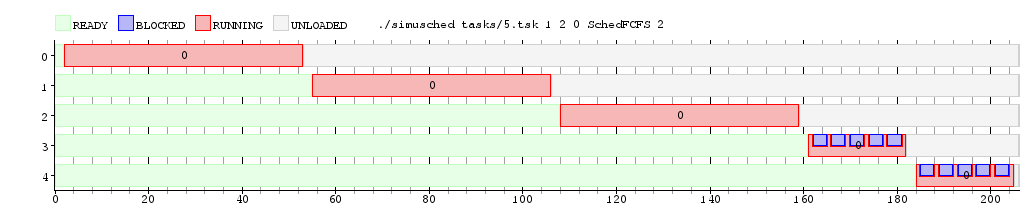
\includegraphics[width=\linewidth]{images/6_quantum2.png}
    \label{fig:Task Consola}
    \caption{FCFS}
\end{figure}

Ya hemos experimentado con este lote bajo el algoritmo de Round-Robin, y con diferentes \textit{quantums} durante el ejercicio anterior. Ahora en esta oportunidad, lo hacemos bajo el algoritmo del scheduler FCFS, y con el mismo lote. La idea es exihibir las diferencias ya advertidas en esta sección entre ambos schedulers. Para empezar, como en el caso anterior, se requieren de 2 ciclos de reloj para cada intercambio de contexto; dandole este tiempo de espera a la primer tarea, de tipo TaskCPU. La diferencia mas notable con la rutina anterior, es que cada tarea no es interrumpida sino hasta que la misma finalice; esto para ciertos lotes de tareas podría traer una penalización severa de performance, pues mientras una tarea realiza una llamada bloqueante, la CPU permanece ociosa hasta que la misma termine, en especial en aquellos casos en que el bloqueo se prolongue por mucho tiempo. En este caso, la mayoria de las tareas del lote son del tipo TaskCPU, que hacen pleno uso del CPU, por lo que el tiempo perdido en los bloqueos cortos de las otras dos tareas se compensan en ahorros que demora conmutar frecuentemente las tareas (lo que ocurre en el Round-Robin), dando una performance parecida o hasta mejor que con el algoritmo de Round-Robin.